\section{Problem Set 2}

\subsection{Everything is Relative}

\subsubsection{Initial Conditions}
For this problem, we use the ISS orbit parameters from Problem Set 1 for the chief spacecraft, and apply small variations to create the deputy spacecraft's initial state:

\begin{table}[H]
    \centering
    \begin{tabular}{ccc} \hline
        \textbf{Parameter} & \textbf{Chief} & \textbf{Deputy} \\ \hline 
        Initial position (RTN) [m] & [0, 0, 0] & [0, 0, 0] \\
        Initial velocity (RTN) [m/s] & [0, 0, 0] & [1, 1, 0] \\ \hline
    \end{tabular}
    \caption{Initial conditions for chief and deputy spacecraft in RTN frame}
    \label{tab:relative_ics}
\end{table}

The deputy begins at the same position as the chief but with a 1 m/s velocity offset in both the tangential and normal directions.

\subsubsection{Nonlinear Equations of Relative Motion}

\begin{figure}[H]
    \centering
    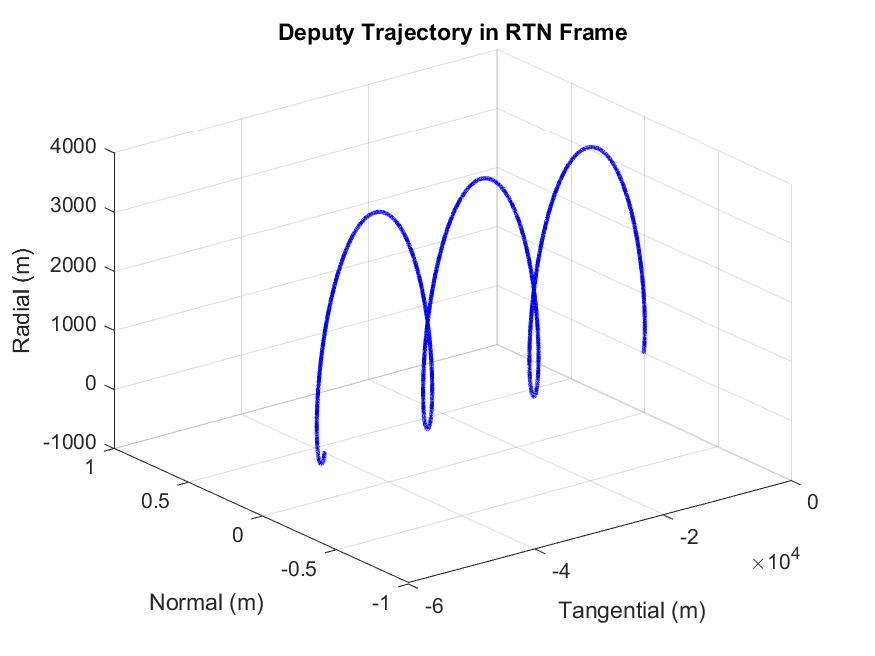
\includegraphics[width=0.7\textwidth]{PS2/Figures/Case1_RelativeTrajectory.png}
    \caption{Deputy trajectory in RTN frame from nonlinear equations of relative motion}
    \label{fig:relative_trajectory}
\end{figure}

\begin{figure}[H]
    \centering
    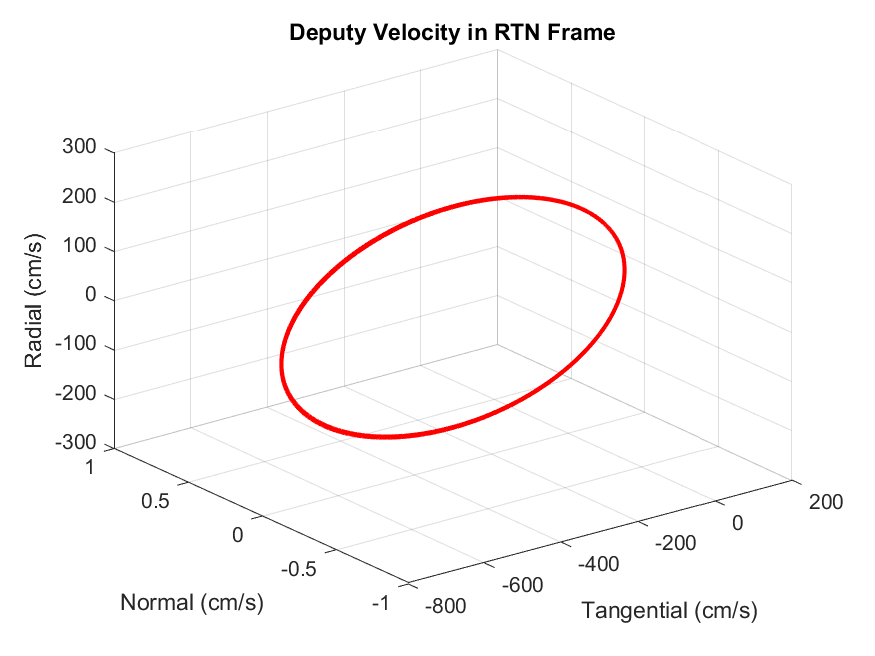
\includegraphics[width=0.7\textwidth]{PS2/Figures/Case1_RelativeVelocity.png}
    \caption{Deputy velocity in RTN frame from nonlinear equations of relative motion}
    \label{fig:relative_velocity}
\end{figure}

\subsubsection{Comparison of Methods}

\begin{figure}[H]
    \centering
    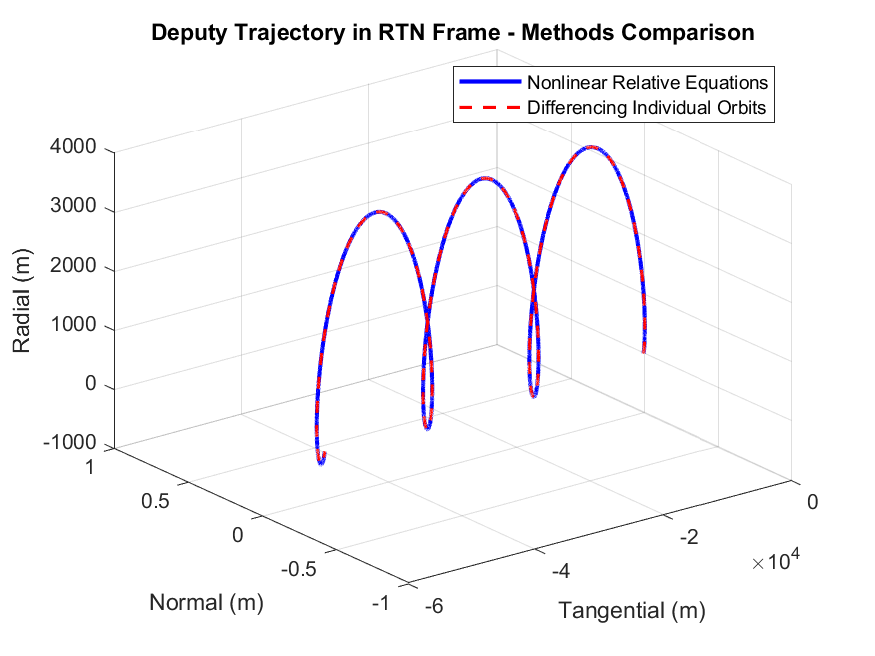
\includegraphics[width=0.7\textwidth]{PS2/Figures/Case1_MethodsComparison.png}
    \caption{Comparison of relative motion computed using nonlinear equations vs. differencing individual orbits}
    \label{fig:methods_comparison}
\end{figure}

\begin{figure}[H]
    \centering
    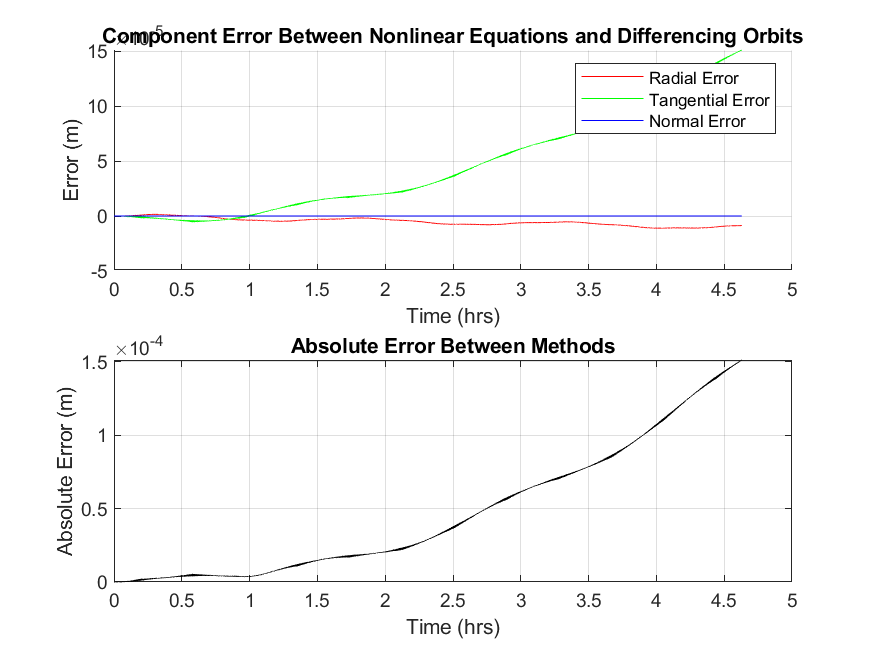
\includegraphics[width=0.7\textwidth]{PS2/Figures/Case1_MethodsError.png}
    \caption{Error between the two methods of computing relative motion}
    \label{fig:methods_error}
\end{figure}

Both methods produce nearly identical results, with maximum errors less than 0.2 mm and mean errors less than 0.05 mm, confirming their mathematical equivalence.

\subsubsection{Effect of Non-Zero Difference in Semi-Major Axis}

When a non-zero difference in semi-major axis is introduced by adding a 1 m/s tangential velocity component to the deputy, in addition to a 1 m/s radial velocity at the start of the simulation, there is drift:

\begin{figure}[H]
    \centering
    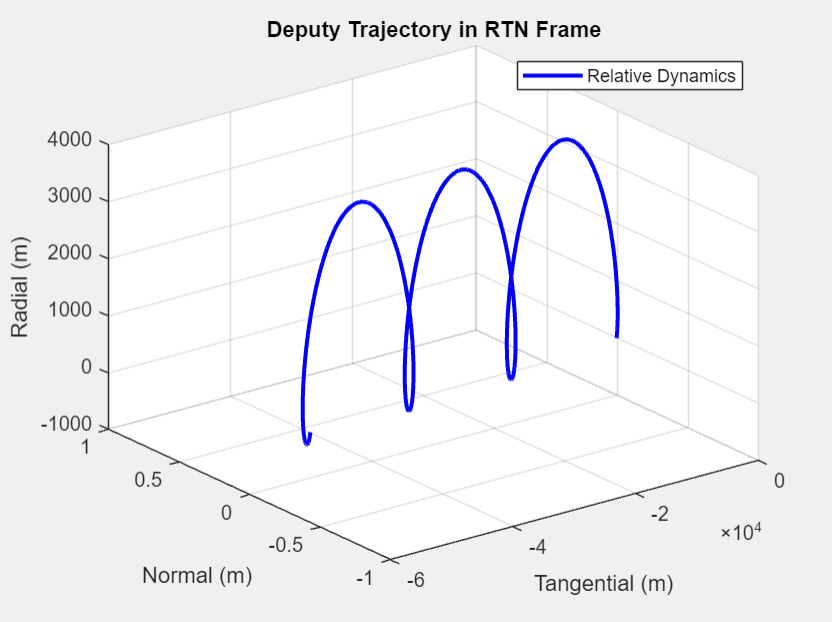
\includegraphics[width=0.7\textwidth]{PS2/Figures/Screenshot 2025-04-16 232749.png}
    \caption{Drifting Orbit}
    \label{fig:drift_comparison}
\end{figure}


\subsubsection{Re-establishing Bounded Motion}

To re-establish bounded periodic motion, we need to eliminate the semi-major axis difference through an impulsive maneuver. The most fuel-efficient approach is a tangential impulse at either apogee or perigee. Our code determines which is more efficent, and applies the manuver at that given point. The results are shown below:

\begin{figure}[H]
    \centering
    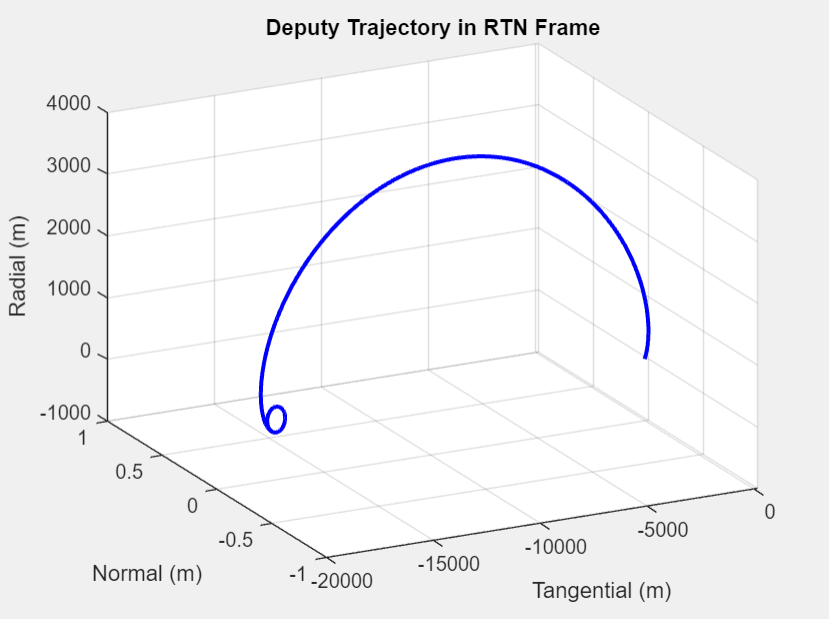
\includegraphics[width=0.7\textwidth]{PS2/Figures/Screenshot 2025-04-16 231907.png}
    \caption{Relative trajectory before and after corrective maneuver}
    \label{fig:maneuver_comparison1}
\end{figure}

\begin{figure}[H]
    \centering
    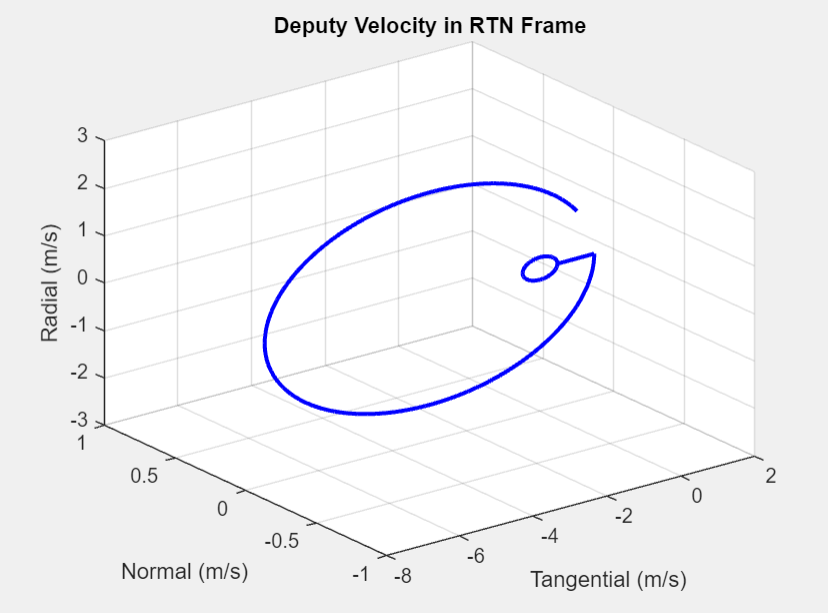
\includegraphics[width=0.7\textwidth]{PS2/Figures/Screenshot 2025-04-16 231937.png}
    \caption{Relative velocity before and after corrective maneuver}
    \label{fig:maneuver_comparison2}
\end{figure}

Analysis of the optimal maneuver:
\begin{itemize}
    \item Maneuver location: Perigee (minimum radius)
    \item Delta-v magnitude: 1.0054 m/s
    \item Maneuver time: 4.29 hours from simulation start
\end{itemize}

This tangential impulse at perigee equalizes the semi-major axes between the chief and deputy, re-establishing bounded relative motion as shown by the post-maneuver trajectory in Figure \ref{fig:maneuver_comparison}. The maneuver is optimal because it changes the orbit energy (and thus semi-major axis) most efficiently by applying thrust in the velocity direction at the point of maximum orbital velocity.

After the maneuver, bounded relative motion is achieved.